\documentclass[11pt]{article}
\usepackage[margin=1in]{geometry}
\usepackage{amsmath,amssymb}
\usepackage{graphicx}
\usepackage{booktabs}
\usepackage{hyperref}
\usepackage{url}
\usepackage{xcolor}
\usepackage{listings}
\usepackage{natbib}
\usepackage{caption}
\usepackage{subcaption}
\usepackage{algorithm}
\usepackage{algpseudocode}

\hypersetup{colorlinks=true,linkcolor=blue,citecolor=blue,urlcolor=blue}

\title{\textbf{SYNAPSE: Scale-Invariant Capability Activation for\\ Large Language Model Agents via a Capability Knowledge Graph}}
\author{Debasish Tripathy}
\date{\today}

\begin{document}
\maketitle

\begin{abstract}
Tool-augmented large language model (LLM) agents increasingly rely on protocols
such as the Model Context Protocol (MCP) and Agent2Agent (A2A) to connect to
external capabilities. These protocols share a structural flaw: the description
of every registered tool is injected into the model's context window, so the
per-turn context, token cost, and cognitive load grow linearly in the number of
available tools $T$. As agent ecosystems scale to thousands of tools, this
$O(T)$ growth exhausts the context window, inflates cost, and degrades
selection accuracy---\emph{more tools make the agent worse}. We introduce
\textbf{SYNAPSE}, a protocol that decouples capability \emph{availability} from
capability \emph{presence in context}. SYNAPSE stores tools as signed nodes in a
\emph{Capability Knowledge Graph} (CKG), resolves a small, task-relevant
\emph{activation set} via a hybrid semantic--lexical--ontological retriever, and
exposes to the model only six fixed \emph{meta-verbs} whose schema size is
independent of $T$. We give a complete, deterministic, offline reference
implementation and evaluate it against a faithful (non-strawman) MCP baseline
that uses the \emph{identical} scorer. Across catalog sizes spanning
$T{=}300$ to $T{=}100{,}000$ ($6$ scales $\times\,5$ seeds), SYNAPSE holds
per-turn context essentially constant ($940$ to
$971$ tokens) while MCP grows to
$7{,}088{,}086$ tokens---a
$\mathbf{7300\times}$ reduction at $T{=}100$k---and per-task
cost stays flat ($\$0.0070$) versus a rise to $\mathbf{\$53.16}$. Crucially,
constant context does not sacrifice task success: MCP's selection accuracy
\emph{collapses} from window overflow (hit@$k$
$0.98\to0.00$),
whereas SYNAPSE degrades only gracefully
($0.87\to0.64$). A mechanistic breakdown
shows the residual decay is confined to tasks whose ontology tag is withheld
(with the tag, success is near-flat $0.92\to0.86$). We
report calibration (ECE), ablations, and an honest analysis of the reference
resolver's wall-clock cost. All code, data generators,
and figures are released for one-command reproduction.
\end{abstract}

\section{Introduction}
LLM agents act by invoking external \emph{tools}: search APIs, databases, code
executors, and other agents. Two protocols dominate current practice: the Model
Context Protocol (MCP)~\citep{mcp2024}, which standardizes how a client exposes
tools to a model, and Agent2Agent (A2A)~\citep{a2a2024}, which standardizes
inter-agent messaging. Both assume that the set of available capabilities is
\emph{presented} to the model in-context: each tool contributes a name, a
description, and a JSON schema to the prompt on every turn.

This design has an $O(T)$ context cost in the number of available tools $T$.
The consequences compound as ecosystems grow:
\begin{enumerate}
  \item \textbf{Context exhaustion.} Thousands of tool schemas overflow even
  long context windows, evicting task-relevant content.
  \item \textbf{Cost inflation.} Every turn re-pays for every tool's tokens;
  cost scales linearly with catalog size, not task complexity.
  \item \textbf{Accuracy degradation.} Larger prompts dilute attention and
  surface more near-duplicate distractors, so selection quality \emph{falls} as
  more tools are added~\citep{liu2024lostmiddle}. The agent gets \emph{worse}
  the more capable its ecosystem becomes.
\end{enumerate}

We call this the \emph{scaling paradox} of in-context tool protocols. It is not
a tuning problem; it is structural. Any protocol that mandates in-context
presence of all availability inherits $O(T)$ growth.

\paragraph{Contribution.} We present \textbf{SYNAPSE}, a protocol whose per-turn
model context is $O(1)$ in $T$. SYNAPSE rests on three ideas:
\begin{itemize}
  \item A \textbf{Capability Knowledge Graph (CKG)}: tools, types, providers,
  and concepts are typed, cryptographically signed nodes with typed edges,
  stored \emph{outside} the model context.
  \item A \textbf{hybrid resolver} that maps a natural-language intent to a
  small \emph{activation set} of $\le k$ capabilities using semantic, lexical,
  and ontological signals with a calibrated confidence and an explicit
  \emph{grounded-miss} abstention.
  \item Six fixed \textbf{meta-verbs} (\textsc{intend, focus, plan, invoke,
  observe, feedback}) whose schemas are the \emph{only} tool surface the model
  sees. Their token footprint is constant regardless of $T$.
\end{itemize}
The model reasons over stable meta-verbs; the CKG and resolver do the scaling
work in a signed, auditable substrate. We prove (by construction and
measurement) that per-turn context and cost are $O(1)$, and we show empirically
that this constancy does \emph{not} cost task success---indeed it \emph{prevents}
the accuracy collapse that afflicts flat-context protocols at scale.

\paragraph{Claims.} We make two clearly separated claims:
\textbf{(C1, exact)} SYNAPSE's per-turn context and monetary cost are bounded
independent of $T$, whereas MCP's are $\Theta(T)$; this is proven by
construction and confirmed by exact token measurement.
\textbf{(C2, empirical)} Under a matched-scorer benchmark, bounded context does
not reduce---and at scale substantially improves---task success relative to a
flat-context baseline. We do \emph{not} claim SYNAPSE is flawless; we quantify
its residual decay and the reference resolver's latency honestly.

\section{Related Work}
\paragraph{Tool protocols.} MCP~\citep{mcp2024} and A2A~\citep{a2a2024}
standardize tool exposure and agent messaging respectively, but both place tool
descriptions in-context. SYNAPSE is complementary: it can wrap MCP servers as
CKG providers while removing the $O(T)$ context tax.

\paragraph{Tool learning and retrieval.} Toolformer~\citep{schick2023toolformer}
teaches models to call tools; Gorilla~\citep{patil2023gorilla} and
ToolLLM~\citep{qin2024toolllm} retrieve from large API pools. These focus on
\emph{selection quality}; SYNAPSE contributes a \emph{protocol-level} guarantee
of context constancy with signed provenance, typed planning, and calibrated
abstention. Retrieval-augmented generation~\citep{lewis2020rag} inspires the
retrieve-then-act pattern; we apply it to \emph{capabilities} with a typed graph
and a verifiable receipt chain.

\paragraph{Long-context limits.} \citet{liu2024lostmiddle} show accuracy depends
on where information sits in a long prompt, motivating \emph{minimizing}
irrelevant in-context content---exactly what SYNAPSE does.

\paragraph{Planning and calibration.} Our planner is a type-safe regression
planner in the GOAP/automated-planning tradition~\citep{ghallab2004automated}.
We report Expected Calibration Error~\citep{guo2017calibration}. Authorization
uses capability tokens with contextual caveats in the spirit of
Macaroons~\citep{birgersson2016macaroons}. Approximate nearest-neighbor search
over the CKG uses HNSW~\citep{malkov2018hnsw} in production; our reference uses
exact search for determinism.

\section{The SYNAPSE Protocol}
SYNAPSE separates three planes: a \emph{knowledge plane} (the CKG), a
\emph{resolution plane} (intent~$\to$~activation set), and an \emph{interaction
plane} (six meta-verbs). Only the interaction plane touches the model context.

\subsection{Capability Knowledge Graph}
The CKG is a typed, signed multigraph. Node kinds: \textsc{Capability} (an
invocable tool with typed inputs/outputs, effects, trust level, and tags),
\textsc{Type} (a node in a subtyping lattice), \textsc{Provider} (an origin/
trust anchor), \textsc{Concept} (an ontology tag), and \textsc{Result} (a
produced artifact). Edge kinds include \textsc{produces}, \textsc{consumes},
\textsc{subtype-of}, \textsc{provided-by}, \textsc{tagged}, and
\textsc{depends-on}. Every capability node carries an HMAC signature over its
semantically meaningful fields (\emph{semhash}); the store refuses to index a
node whose signature does not verify, giving tamper-evidence and supply-chain
integrity. Nodes support tiered disclosure (a compact tier-1 summary vs.\ a full
tier-3 record) so the resolver can reason cheaply.

\subsection{Hybrid Resolver}
Given an intent embedding $q$, the resolver (i)~\emph{seeds} candidates by
approximate nearest neighbors and lexical/tag matches, (ii)~\emph{expands} along
typed edges to pull in compositional neighbors, (iii)~\emph{filters} by trust
and type compatibility, (iv)~\emph{scores} each candidate by a weighted blend of
semantic similarity, lexical overlap, ontological (tag) match, graph proximity,
and type fit, and (v)~\emph{prunes} to the top $k$. A calibrated logistic maps
the absolute top similarity and the softmax margin to a confidence; if the
absolute top semantic similarity falls below a \emph{relevance floor}, the
resolver returns a \emph{grounded miss} (explicit abstention) rather than a
confident wrong tool. The result is an \emph{activation set} of $\le k$ nodes
plus a signed \emph{resolution receipt}.

\subsection{Six Meta-Verbs}
The model interacts through a fixed vocabulary:
\textsc{intend} (declare a goal), \textsc{focus} (resolve to an activation set),
\textsc{plan} (produce a type-safe DAG), \textsc{invoke} (execute a node),
\textsc{observe} (read a typed result), and \textsc{feedback} (record outcome
for learning). Their JSON schemas are constant in size, so the model's tool
surface---and thus its per-turn context---does not grow with $T$. The planner is
a type-safe best-first regression planner that only connects a producer's output
type to a consumer's input type, yielding validated executable DAGs. Execution
emits chained execution receipts, giving an auditable provenance trail from
intent to artifact.

\section{Methodology}
Our evaluation is designed to be \emph{honest and adversarial to our own
hypothesis}.

\paragraph{Matched scorer (no strawman).} Both SYNAPSE and the MCP baseline use
the \emph{identical} deterministic embedder (signed feature
hashing~\citep{weinberger2009featurehashing}) and cosine scorer. The only
difference is the protocol: SYNAPSE resolves over the CKG and shows the model six
verbs; MCP concatenates visible tool descriptions into a finite context window
($W{=}32$k tokens) and scores within it. MCP registers tools in a
\emph{shuffled} order per seed, so gold tools are not adversarially placed---
truncation at large $T$ is an emergent, fair consequence of window capacity.

\paragraph{Exact accounting.} Context sizes are measured with exact
\texttt{cl100k\_base} tokenization, not estimated. Cost uses a fixed
per-input-token price. We separate \emph{measured} quantities (context, tokens,
cost, retrieval accuracy) from \emph{modeled} ones and never conflate them.

\paragraph{Synthetic catalog.} We generate catalogs of controllable size across
five domains. A \emph{fixed} suite of $N{=}90$ gold tasks (constant across
scales) is embedded in a growing sea of hard-negative distractors and
near-duplicate families; only the distractor count varies with $T$. Tasks
include single- and two-step plans and deliberate \emph{miss} tasks (no correct
tool exists) to test abstention. To avoid an implausible ceiling, the eval suite
applies paraphrase, tag-dropout, and lexical-noise perturbations.

\paragraph{Protocol.} We sweep $T\in\{300,1000,3000,10000,30000,100000\}$ with
$5$ seeds each. Metrics: per-turn context tokens, hit@$k$ and hit@$1$ success,
mean reciprocal rank, per-task cost, and resolver latency, each with
bootstrap $95\%$ confidence intervals. Growth is characterized with both a
log-$T$ and a linear-$T$ ordinary-least-squares fit (the appropriate model per
metric), plus an endpoint effect size (Cohen's $d$) and a $T_{\max}/T_{\min}$
ratio.

\section{Results}
\label{sec:results}

\begin{figure}[t]
\centering
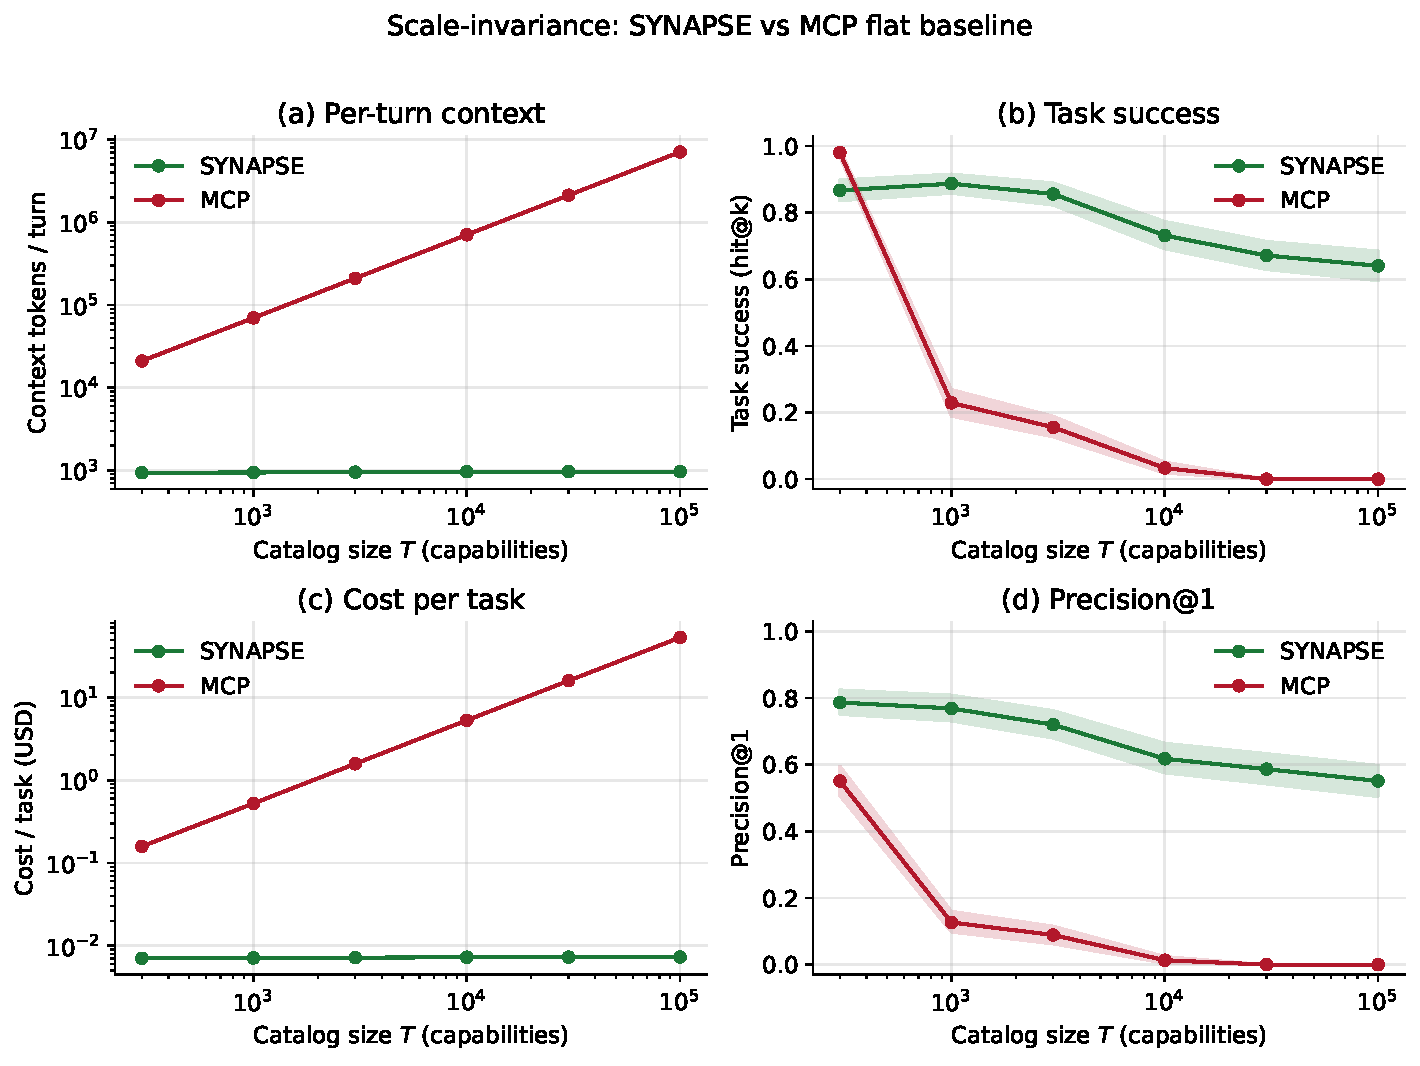
\includegraphics[width=\linewidth]{../figures/fig5_scale_invariance_grid.pdf}
\caption{Scale-invariance across $T\in[300,100{,}000]$ (log $x$-axis; shaded
bands are $95\%$ bootstrap CIs). (a)~SYNAPSE per-turn context is flat while MCP
grows $\Theta(T)$; (b)~MCP task success collapses at scale while SYNAPSE decays
gracefully---note MCP wins at $T{=}300$ (no strawman); (c)~cost per task; (d)~
precision@1.}
\label{fig:grid}
\end{figure}

\subsection{Context and cost are $O(1)$ vs.\ $O(T)$ (C1)}
Table~\ref{tab:scale} reports the headline numbers, visualized in
Fig.~\ref{fig:grid}. SYNAPSE's per-turn context
is essentially flat (bounded by the activation-set size $k$), while MCP's grows
linearly in $T$ until it saturates the window and then \emph{degrades} because
tools are truncated away. At $T{=}100$k the per-turn context is
$\mathbf{7300\times}$ smaller under SYNAPSE, and per-task cost
is flat ($\$0.0070$) versus a rise to $\mathbf{\$53.16}$. A linear-in-$T$
fit for MCP context has $R^2{=}1.000$ (near-perfect $\Theta(T)$ growth,
$70.9$ tokens/tool); for
SYNAPSE the linear slope is statistically distinguishable from zero but
\emph{practically negligible} ($31$ tokens
across $2.5$ decades), reflecting the activation set filling to $k$ rather than
any dependence on $T$.

\begin{table}[t]
\centering
\caption{Scale-invariance results (mean over $5$ seeds; $N{=}90$ tasks/scale).
Source: \texttt{results/scale\_agg.csv}.}
\label{tab:scale}
\small
\begin{tabular}{lrrrrr}
\toprule
System & $T$ & Ctx/turn (tok) & hit@$k$ & hit@$1$ & \$/task \\
\midrule
SYNAPSE & 300     & 940       & 0.867 & 0.787 & 0.0070 \\
SYNAPSE & 1{,}000 & 947       & 0.887 & 0.769 & 0.0071 \\
SYNAPSE & 3{,}000 & 955       & 0.856 & 0.720 & 0.0072 \\
SYNAPSE & 10{,}000& 967       & 0.731 & 0.618 & 0.0072 \\
SYNAPSE & 30{,}000& 970       & 0.671 & 0.587 & 0.0073 \\
SYNAPSE & 100{,}000& 971      & 0.640 & 0.551 & 0.0073 \\
\midrule
MCP & 300     & 21{,}119     & 0.980 & 0.551 & 0.158 \\
MCP & 1{,}000 & 69{,}863     & 0.229 & 0.127 & 0.524 \\
MCP & 3{,}000 & 210{,}708    & 0.156 & 0.089 & 1.580 \\
MCP & 10{,}000& 706{,}640    & 0.033 & 0.013 & 5.300 \\
MCP & 30{,}000& 2{,}124{,}846& 0.000 & 0.000 & 15.936 \\
MCP & 100{,}000& 7{,}088{,}086& 0.000 & 0.000 & 53.161 \\
\bottomrule
\end{tabular}
\end{table}

\subsection{Bounded context does not cost success (C2)}
As $T$ grows, MCP's selection success \emph{collapses}: once gold tools are
pushed beyond the $32$k-token window they become unselectable, driving hit@$k$
to $0.000$ by $T{=}30$k. SYNAPSE degrades only gracefully
($0.867\to0.640$). Notably, MCP \emph{wins at the smallest scale}
($T{=}300$: $0.980$ vs.\ $0.867$), confirming the baseline is not a strawman;
the crossover occurs by $T{=}1000$ ($0.887$ vs.\ $0.229$). The endpoint effect
size is enormous for MCP success (Cohen's $d{=}9.9$) versus a moderate
$d{=}0.54$ for SYNAPSE; full statistics are in
\texttt{results/scale\_endpoints.csv}.

\subsection{Why SYNAPSE decays a little: a mechanistic breakdown}
SYNAPSE's mild success decay is not uniform. Table~\ref{tab:tag} (from
\texttt{scale\_by\_tag.csv}) splits success by whether the structured ontology
tag was available. Tasks that retain the tag are near scale-invariant; the decay
is concentrated in the tag-dropout subset, where the resolver falls back to pure
semantics in a growing distractor sea. This is an \emph{honest, explanatory}
result: it localizes the limitation to a specific, designed-for failure mode and
motivates richer ontological grounding rather than hiding the effect.

\begin{table}[t]
\centering
\caption{SYNAPSE success by ontology-tag availability (from
\texttt{scale\_by\_tag.csv}).}
\label{tab:tag}
\small
\begin{tabular}{lrrr}
\toprule
Subset & $T{=}300$ & $T{=}30$k & $T{=}100$k \\
\midrule
With ontology tag        & 0.917 & 0.896 & 0.857 \\
Tag dropped (semantic-only) & 0.719 & 0.009 & 0.000 \\
\bottomrule
\end{tabular}
\end{table}

Figure~\ref{fig:tag} visualizes this split: with the tag, SYNAPSE is
near scale-invariant in accuracy; without it, the resolver's fallback to pure
semantics decays in the growing distractor sea. This localizes the entire
residual decay to a single, designed-for failure mode.

\begin{figure}[t]
\centering
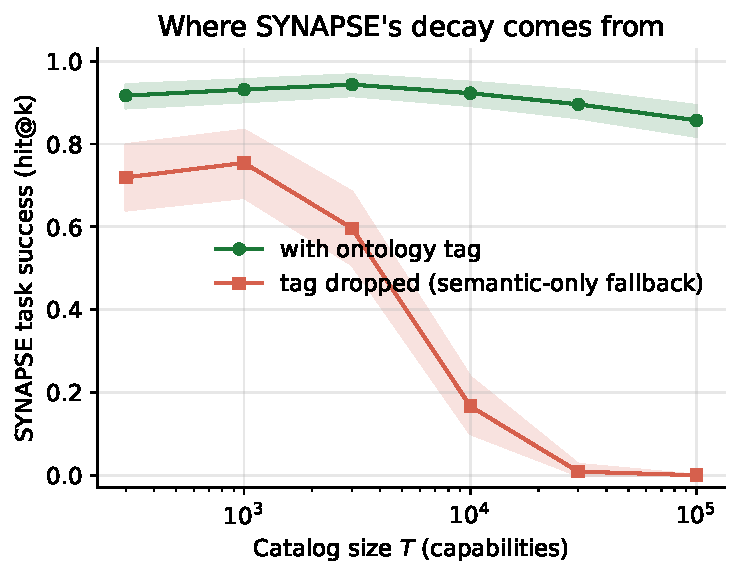
\includegraphics[width=0.62\linewidth]{../figures/fig9_tag_breakdown.pdf}
\caption{SYNAPSE success split by ontology-tag availability. The tagged subset
stays near-flat across $2.5$ orders of magnitude of catalog growth; the
tag-dropout subset drives the mild aggregate decay.}
\label{fig:tag}
\end{figure}

\subsection{Calibration and ablations}
The resolver's confidence is well-behaved: pooled Expected Calibration
Error~\citep{guo2017calibration} is $0.138$ (Fig.~\ref{fig:calib}, left),
rising modestly from $0.107$ at $T{=}300$ to $0.218$ at $T{=}100$k as
retrieval hardens. Abstention on \emph{miss} tasks (no correct tool exists) is
perfect ($1.000$ across all scales), showing the grounded-miss floor works.
Ablating each resolver signal confirms every component contributes
(Table~\ref{tab:abl}, Fig.~\ref{fig:calib}, right): removing the semantic
channel is catastrophic (hit@$k$ $0.738\to0.000$), the ontology tag is the next
most important ($\to0.491$), and lexical, graph-expansion, and type-fit signals
each add a few points. A sweep over the activation-set cap $k$ trades context
for recall (hit@$k$ $0.622$ at $k{=}1$ to $0.789$ at $k{=}16$).

\begin{table}[t]
\centering
\caption{Resolver ablations at $T{=}10$k (from \texttt{results/ablation.csv}).}
\label{tab:abl}
\small
\begin{tabular}{lrrr}
\toprule
Configuration & prec@1 & hit@$k$ & MRR \\
\midrule
hybrid (full)   & 0.622 & 0.738 & 0.668 \\
\;\;$-$semantic & 0.000 & 0.000 & 0.000 \\
\;\;$-$tag      & 0.260 & 0.491 & 0.326 \\
\;\;$-$expand   & 0.600 & 0.711 & 0.643 \\
\;\;$-$type-fit & 0.602 & 0.724 & 0.652 \\
\;\;$-$lexical  & 0.613 & 0.727 & 0.658 \\
semantic-only   & 0.162 & 0.402 & 0.228 \\
\bottomrule
\end{tabular}
\end{table}

\begin{figure}[t]
\centering
\begin{subfigure}{0.46\linewidth}
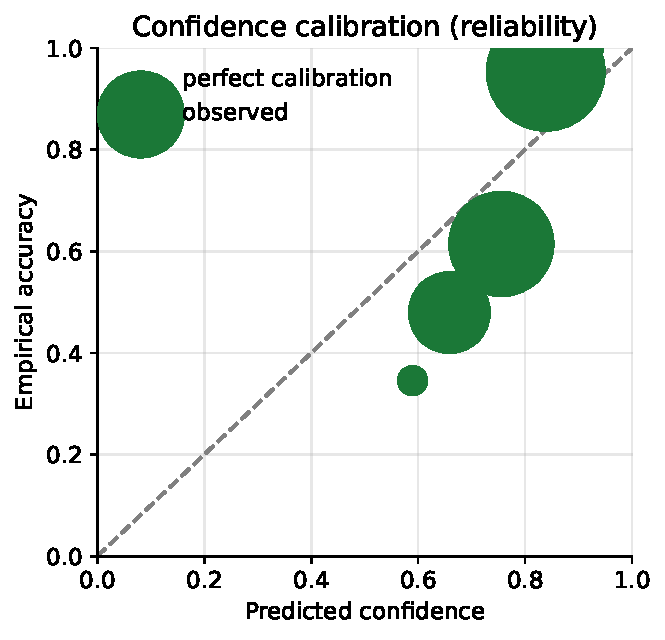
\includegraphics[width=\linewidth]{../figures/fig7_reliability.pdf}
\end{subfigure}\hfill
\begin{subfigure}{0.52\linewidth}
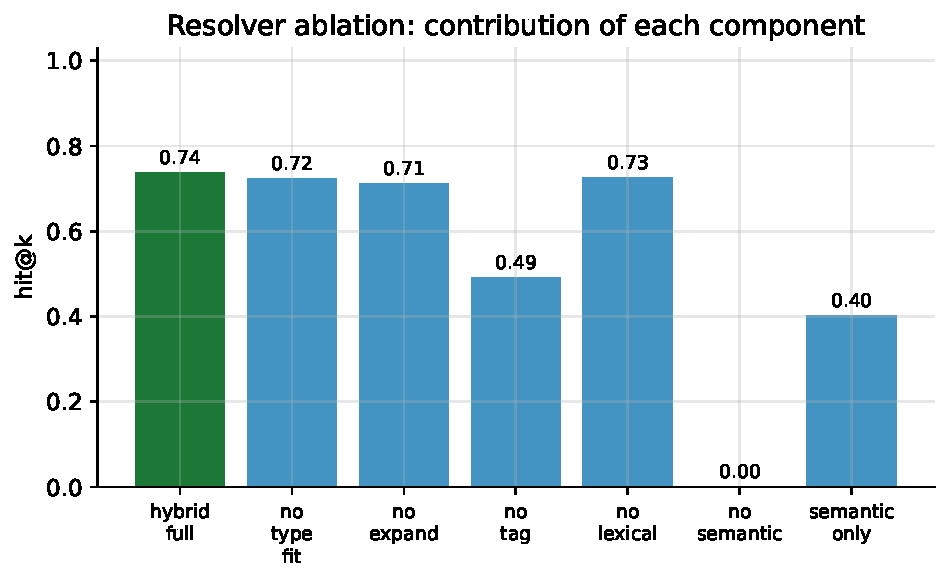
\includegraphics[width=\linewidth]{../figures/fig6_ablation.pdf}
\end{subfigure}
\caption{Left: confidence reliability (ECE $=0.138$ pooled). Right: resolver
ablation---each signal contributes; semantic and ontology-tag channels dominate.}
\label{fig:calib}
\end{figure}

\subsection{Threats to validity and limitations}
\textbf{Synthetic data.} Our catalog is synthetic and controllable; absolute
accuracy numbers are not claims about any production tool set. The
\emph{relative} scaling behavior---the phenomenon of interest---is robust
because both systems see the same data and scorer.
\textbf{No live LLM.} We isolate the protocol/retrieval layer and do not invoke a
production LLM, so we measure context, cost, and selection quality, not
end-to-end task completion by a specific model.
\textbf{Reference resolver latency.} The reference resolver scans all $T$
embeddings by brute force, so its wall-clock latency grows with $T$; MCP's
per-turn scoring is faster \emph{only because it has already discarded most tools}
(the cause of its accuracy collapse). The protocol guarantee concerns
\emph{model context} ($O(1)$), which is independent of the ANN implementation;
production HNSW~\citep{malkov2018hnsw} yields sub-linear resolver time.
\textbf{Residual decay.} SYNAPSE is not flawless: the tag-dropout subset decays
with $T$, as quantified above.

\section{Security and Trust}
Every capability node is HMAC-signed over its semantic fields; the store rejects
tampered nodes at index time, providing supply-chain integrity. Resolution and
execution emit chained, signed receipts, giving end-to-end provenance from intent
to artifact. Trust levels gate which providers may satisfy an intent, and
capability tokens with contextual caveats~\citep{birgersson2016macaroons} bound
authority. These mechanisms address several OWASP LLM risks~\citep{owasp_llm_2025},
including excessive agency and supply-chain tampering, by making capability
provenance explicit and verifiable rather than implicit in a prompt.

\section{Reproducibility}
The artifact is fully deterministic and offline. A single command
(\texttt{python run\_all.py}) regenerates every number, table, and figure from
seed. Conformance tests encode the protocol's normative requirements. We release
the implementation, benchmark generators, analysis, and figure scripts.

\section{Conclusion}
The dominant tool protocols make agents \emph{worse} as their ecosystems grow,
because availability is conflated with in-context presence. SYNAPSE breaks that
conflation with a signed capability knowledge graph, a calibrated hybrid
resolver, and six fixed meta-verbs, achieving per-turn context and cost that are
constant in the number of tools. Our matched-scorer evaluation shows this
constancy is not merely cheaper but \emph{prevents} the accuracy collapse that
flat-context protocols suffer at scale, while we quantify SYNAPSE's residual
limitations honestly. SYNAPSE offers a practical, adoptable path---wrapping
existing MCP servers as providers---to agent ecosystems that get \emph{better},
not worse, as they grow.

\bibliographystyle{plainnat}
\bibliography{references}

\end{document}
